%!TEX root = ../report_template.tex
\section{Results and Discussion}
The introduced student-to-teacher ratio combines the number of children with the number of teachers, either for each federal state or school type.
% This section will compare it to the Abitur grades, repeaters, and budgets.
Thus, this section compares the student-to-teacher ratio with the Abitur grades, repeaters, and budgets. 
% Due to how the data is represented, the Abitur grades can only be analyzed for the German average.
Importantly, the Abitur grades can only be analyzed for the German average, due to the missing representation. Nevertheless, the repeaters and budgets are analyzed for each federal state.

One of the key findings of this analysis is the strong correlation between the average grades across all federal states and the student-to-teacher ratio in German grammar schools. As shown in \autoref{fig:regression-stt-grade}, the relationship between both is nearly linear and contains neither clusters nor outliers. 
% Hence -> Thus
Hence, a smaller student-to-teacher ratio strongly correlates to better Abitur grades, with a Pearson correlation coefficient of $0.98$.

\begin{figure}[ht]
    \centering
    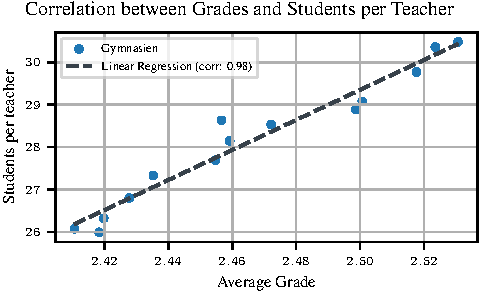
\includegraphics{fig/fig_correlation_grades_students_per_teacher.pdf}
    \caption{Linear regression on the student-to-teacher ratio by average Abitur grade. The resulting regression line (\textcolor{TUred}{\rule[-0.2ex]{0.5em}{2pt} \rule[-0.2ex]{0.5em}{2pt}}) is calculated over the aggregated average overall grammar schools (\textcolor{TUlightblue}{\tikz\draw[fill={TUlightblue}] (0,0) circle (0.25em);}) in Germany.}
    \label{fig:regression-stt-grade}
\end{figure}

% This confirms ... and is consistent with the findings of prior research \cite...
% (a correlation is technically not a result, as in 'the result of some complicated computation or the return value of an algorithm', but just a different way of representing the given data)
This result confirms the initial hypothesis of the big influence of the student-to-teacher ratio and is consistent with studies in other countries \cite{kasau_onesmus_mulei_pupil-teacher_2016,koc_impact_2015,dickson_economic_1984}.

% ...only give...
However, the Abitur grades give only an insight into grammar schools. 
% So additionally, the...
Thus, the correlations with repeaters and budgets are shown in \autoref{fig:heatmap_correlation_students_per_teacher_repeaters_budget}. 
% this sentence doesn't convey info that is not already in the heatmap
% and the heatmap is already explained in the caption
% => the sentence can be removed
It presents a visualization of the Pearson correlation coefficients, analyzing the relationship between the number of children per teacher and the average number of repeaters, as well as the educational budget per child. 
% 'Therefore' implies a causal relationship that does not exist. consider replacing with smth like 'Note that'
Therefore, the Pearson correlation coefficients for each state are normalized to the used color map scale.

\begin{figure}[ht]
    \centering
    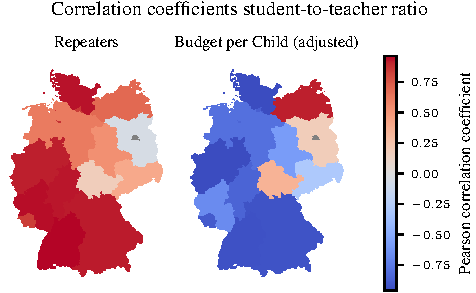
\includegraphics{fig/fig_heatmap_correlation_students_per_teacher_repeaters_budget.pdf}
    \caption{Pearson correlation coefficients between the student-to-teacher ratio and the relative repeater count (left) and the inflation-adjusted average budget per child (right). \textcolor{red}{Red} indicates positive, \textcolor{gray}{light gray} neutral, \textcolor{TUdark}{gray} missing, and \textcolor{blue}{blue} negative correlations between the variables.}
    \label{fig:heatmap_correlation_students_per_teacher_repeaters_budget}
\end{figure}

% represented -> presented/shown 
The findings represented in \autoref{fig:heatmap_correlation_students_per_teacher_repeaters_budget} support a  positive correlation between the student-to-teacher ratio and the number of repeaters in most federal states. 
% in contrast to what? we are still talking about one and the same figure! make sure the reader knows you are talking about the two heatmaps in the figure
In contrast, they indicate a negative correlation between the student-to-teacher ratio  and budget per child for the same states. Furthermore, there is a big difference between \emph{old} and \emph{new} federal states for both correlations. Especially, the results for Thüringen and Brandenburg diverge from the average in both maps. Rather, Mecklenburg-Vorpommern differs most in the budget per child from the other states.

However,  an increase in the number of students in the new federal states can explain the different correlations in the budget per child\footref{footnote:teachers-children}. Since the per-child budget has increased in all states\footref{footnote:budget}, the schools got more cash in total. This results in more vacancies at schools \cite{kultusminister_konferenz_lehrkrafteeinstellungsbedarf_2023} and other investments, like digitalization and maintenance of schools \cite{bundesministerium_fur_bildung_und_forschung_fortschrittsbericht_2022}. But in the short term, there will be more teachers needed as available \cite{kultusminister_konferenz_lehrkrafteeinstellungsbedarf_2023}. As \autoref{fig:teacher_contracts} indicates, this leads to a high variance in the distribution of teacher contract types, especially for the new federal states. This results in a higher student-to-teacher ratio with the same budget.

In contrast, the anomaly for the repeaters involves more aspects of the educational system, like the different curricula or conditions for repeating a class. The importance attached to repetition varies from federal state to federal state and cannot necessarily be used as an indicator of educational quality \cite{klemm_klassenwiederholungen_2009}. Hence, a complete explanation for these results involves more datasets and effects, which are not analyzed in this paper.

Moreover, all other states indicate that a higher budget per child results in a smaller student-to-teacher ratio. As a result, the number of repeaters decreases with the student-to-teacher ratio.